\documentclass[11pt,a4paper]{article}

\usepackage[utf8]{inputenc}
\usepackage[T1]{fontenc}
\usepackage{lmodern}
\usepackage{graphicx}
\usepackage{xcolor}
\usepackage{hyperref}
\usepackage{geometry}
\usepackage{booktabs}
\usepackage{listings}
\usepackage{tcolorbox}
\usepackage{tikz}
\usepackage{needspace}
\usetikzlibrary{shapes.geometric, arrows, positioning, shadows, fit, calc}

\geometry{margin=1in}

% Style adjustments for continuous flow
\usepackage{titlesec}
\titleformat{\section}{\Large\bfseries\color{primary}}{\thesection}{1em}{}
\titleformat{\subsection}{\large\bfseries\color{primary}}{\thesubsection}{1em}{}
\titleformat{\subsubsection}{\normalsize\bfseries\color{secondary}}{\thesubsubsection}{1em}{}

\definecolor{primary}{RGB}{0, 102, 204}
\definecolor{secondary}{RGB}{102, 102, 102}
\definecolor{codebg}{RGB}{245, 245, 245}
\definecolor{cmdcolor}{RGB}{0, 128, 0}
\definecolor{warning}{RGB}{200, 0, 0}

\hypersetup{
    colorlinks=true,
    linkcolor=primary,
    filecolor=magenta,      
    urlcolor=primary,
    pdftitle={XDP-L2-Guard: Deep Technical Manual},
    pdfpagemode=UseNone,
}

\lstset{
    backgroundcolor=\color{codebg} ,
    basicstyle=\ttfamily\small,
    breaklines=true,
    frame=single,
    rulecolor=\color{secondary},
    keywordstyle=\color{primary},
    commentstyle=\color{secondary},
    stringstyle=\color{cmdcolor},
    captionpos=b,
    keepspaces=true,
}

\title{\textbf{XDP-L2-Guard: Comprehensive Engineering Manual \\ \large High-Performance Layer-2 \& Layer-3 Traffic Orchestration with eBPF/XDP}}
\author{Platform Engineering Team}
\date{\today}

\begin{document}

\maketitle

\begin{abstract}
XDP-L2-Guard is a high-performance, programmable network orchestration filter leveraging the Linux eXpress Data Path (XDP). Operating directly inside the Network Interface Card (NIC) driver hook, it provides sub-microsecond packet processing capabilities for Layer-2 and Layer-3 traffic. This enables wire-speed dropping, packet redirection, hairpinning, and state-aware Network Address Translation (NAT) before the Linux kernel allocates socket buffers (\texttt{sk\_buff}). This manual serves as an exhaustive, low-level technical reference covering C-level memory structures, Python CO-RE management, checksum algorithms, and deployment strategies.
\end{abstract}

\tableofcontents
\vspace{1cm}

\section{System Architecture and Paradigm}

The system is strictly architected around the paradigm of control/data plane separation. The **Data Plane** is written in restricted C, compiled via Clang/LLVM into eBPF bytecode, and executes securely within the kernel context. The **Control Plane** utilizes Python 3 to orchestrate the lifecycle of the eBPF program, utilizing \texttt{iproute2} and \texttt{bpftool} to manage asynchronous state updates.

\subsection{Architectural Component Diagram}

\begin{center}
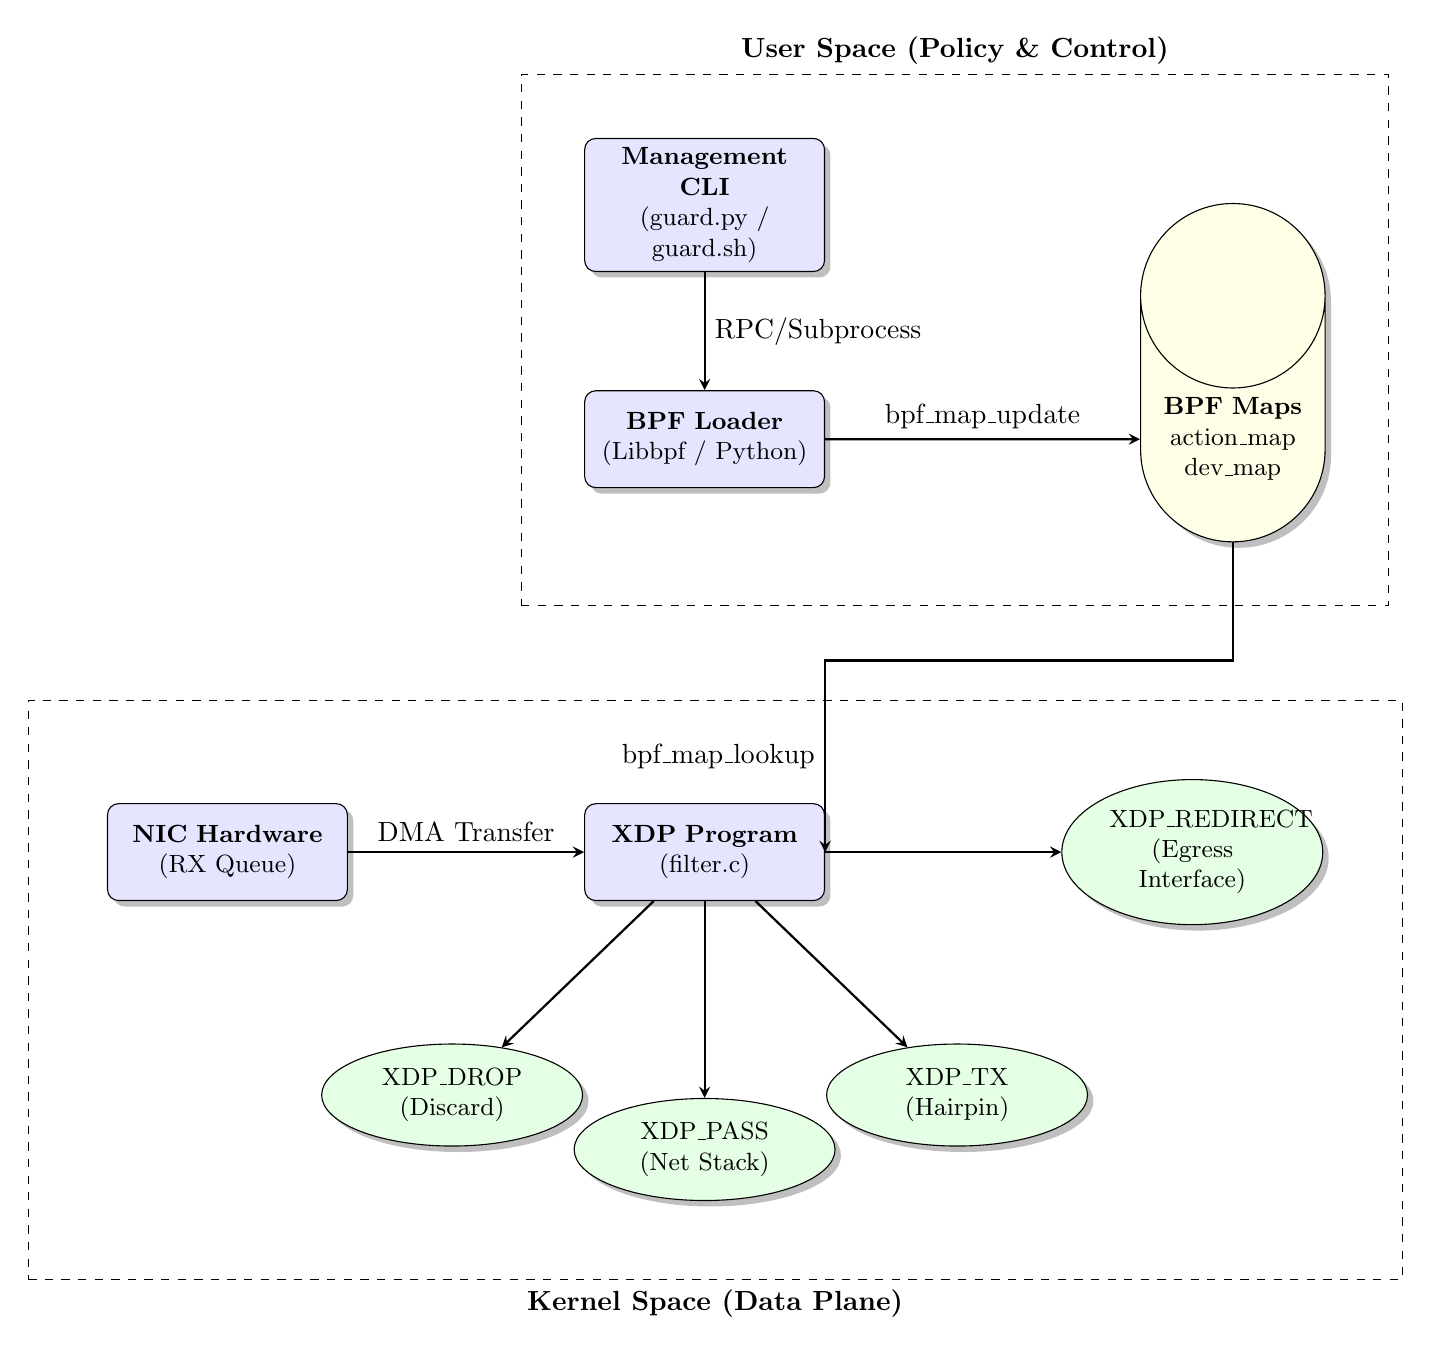
\begin{tikzpicture}[
    node distance=3cm,
    block/.style={rectangle, draw, fill=blue!10, text width=8em, text centered, rounded corners, minimum height=3.5em, drop shadow, font=\small},
    map/.style={cylinder, draw, fill=yellow!10, text width=6em, text centered, shape border rotate=90, minimum height=4.5em, drop shadow, font=\small},
    cloud/.style={draw, ellipse, fill=green!10, text width=6em, text centered, minimum height=3em, drop shadow, font=\small},
    arrow/.style={thick,->,>=stealth}
]

% User Space Components
\node [block] (cli) {\textbf{Management CLI} \\ (guard.py / guard.sh)};
\node [block, below=1.5cm of cli] (loader) {\textbf{BPF Loader} \\ (Libbpf / Python)};
\node [map, right=4cm of loader] (maps) {\textbf{BPF Maps} \\ action\_map \\ dev\_map};

\node[draw, dashed, inner sep=0.8cm, label={[font=\bfseries]above:User Space (Policy \& Control)}] (userspace) [fit=(cli) (loader) (maps)] {};

% Kernel Space Components
\node [block, below=4cm of loader] (filter) {\textbf{XDP Program} \\ (filter.c)};
\node [block, left=3cm of filter] (nic) {\textbf{NIC Hardware} \\ (RX Queue)};

\node [cloud, below left=2cm and 0.5cm of filter] (discard) {XDP\_DROP \\ (Discard)};
\node [cloud, below=2.5cm of filter] (stack) {XDP\_PASS \\ (Net Stack)};
\node [cloud, below right=2cm and 0.5cm of filter] (bounce) {XDP\_TX \\ (Hairpin)};
\node [cloud, right=3cm of filter] (redirect) {XDP\_REDIRECT \\ (Egress Interface)};

\node[draw, dashed, inner sep=1cm, label={[font=\bfseries]below:Kernel Space (Data Plane)}] (kernel) [fit=(filter) (nic) (discard) (stack) (bounce) (redirect)] {};

% Explicit Logical Connections
\draw [arrow] (cli) -- node[right] {RPC/Subprocess} (loader);
\draw [arrow] (loader) -- node[above] {bpf\_map\_update} (maps);
\draw [arrow] (maps.south) -- ++(0,-1.5) -| node[near end, left] {bpf\_map\_lookup} (filter.east);
\draw [arrow] (nic) -- node[above] {DMA Transfer} (filter);

\draw [arrow] (filter) -- (discard);
\draw [arrow] (filter) -- (stack);
\draw [arrow] (filter) -- (bounce);
\draw [arrow] (filter) -- (redirect);

\end{tikzpicture}
\end{center}

\section{Data Plane Implementation (eBPF/XDP)}

The data plane code (\texttt{src/data\_plane/filter.c}) hooks into the NIC's NAPI poll loop via the \texttt{SEC("xdp")} macro. The function \texttt{xdp\_drop\_logic} acts as the primary ingress orchestrator.

\subsection{Memory Layout and Pointer Validation}

eBPF programs operate in a verified environment. Before the verifier allows access to packet memory, the code must prove that the memory bounds are safe. The program receives a \texttt{struct xdp\_md} context, providing DMA mapped pointers:

\begin{lstlisting}[language=C]
void *data = (void *)(long)ctx->data;
void *data_end = (void *)(long)ctx->data_end;
\end{lstlisting}

We utilize a custom \texttt{BOUNDS\_CHECK} macro defined in \texttt{headers.h}:
\begin{lstlisting}[language=C]
#define BOUNDS_CHECK(pointer, type, data_end) \
    do { \
        if ((void *)(pointer) + sizeof(type) > (void *)(data_end)) \
            return XDP_PASS; \
    } while(0)
\end{lstlisting}

The parsing pipeline proceeds strictly layer by layer:
\begin{enumerate}
    \item \textbf{Layer 2 (Ethernet)}: Cast \texttt{data} to \texttt{struct ethhdr}. Verify bounds. Check if \texttt{eth->h\_proto == bpf\_htons(ETH\_P\_IP)}. If not, bypass to kernel via \texttt{XDP\_PASS}.
    \item \textbf{Layer 3 (IPv4)}: Cast \texttt{data + sizeof(struct ethhdr)} to \texttt{struct iphdr}. Verify bounds. Extract the Destination IP (\texttt{ip->daddr}).
\end{enumerate}

\subsection{Action Map Schema}

The extracted IP is used as a lookup key in the primary BPF hash map, \texttt{action\_map}. The map expects an IPv4 address in network byte order (\texttt{\_\_u32}) and returns a \texttt{struct action\_cfg}:

\begin{lstlisting}[language=C]
struct action_cfg {
    __u32 target;           // 0: PASS, 1: DROP, 2: TX, 3: REDIRECT, 4: NAT
    __u32 new_ip;           // Destination IP for NAT scenarios
    __u32 ifindex;          // OS Interface index for REDIRECT
    __u64 dropped_packets;  // Atomic performance counter
};
\end{lstlisting}

\subsection{Low-Level Action Semantics}

Depending on the retrieved \texttt{target}, the kernel executes one of the following routines:

\subsubsection{XDP\_DROP (Wire-Speed Discard)}
The simplest and fastest action. The NIC driver drops the frame and immediately recycles the DMA buffer. The code atomically increments the global array map \texttt{total\_dropped} and the rule-specific \texttt{dropped\_packets}.

\subsubsection{XDP\_TX (Hairpinning \& ICMP Echo Conversion)}
\texttt{XDP\_TX} bounces the packet back out of the interface it arrived on. In our implementation, this is used for advanced ICMP manipulation. If an \texttt{ICMP\_ECHO} (Ping) is detected:
\begin{enumerate}
    \item The type is rewritten to \texttt{ICMP\_ECHOREPLY} (0).
    \item \textbf{Checksum Math}: Because Type 8 changed to Type 0, the 16-bit 1's complement checksum must be incrementally updated by adding \texttt{0x0800}.
    \item MAC and IP addresses are swapped utilizing \texttt{\_\_builtin\_memcpy} for optimal inline compilation.
\end{enumerate}

\subsubsection{XDP\_REDIRECT \& ACTION\_NAT (DNAT)}
\texttt{ACTION\_NAT} performs Destination Network Address Translation directly in hardware. 
\begin{lstlisting}[language=C]
__u32 old_daddr = ip->daddr;
__u32 new_daddr = cfg->new_ip;
__u32 csum = ~bpf_ntohs(ip->check) & 0xFFFF;
csum += (~(old_daddr & 0xFFFF) & 0xFFFF) + (new_daddr & 0xFFFF);
csum += (~(old_daddr >> 16) & 0xFFFF) + (new_daddr >> 16);
while (csum >> 16) csum = (csum & 0xFFFF) + (csum >> 16);
ip->check = bpf_htons(~csum & 0xFFFF);
\end{lstlisting}
This bitwise logic incrementally updates the IP header checksum without requiring a full packet recalculation, ensuring sub-microsecond latency. \texttt{XDP\_REDIRECT} follows the exact same logic but concludes by forwarding the frame to an interface indexed in \texttt{dev\_map}.

\section{Control Plane: Orchestration and Polling}

The Control Plane comprises two primary Python scripts: \texttt{loader.py} for lifecycle management and \texttt{guard.py} for CLI rule definition.

\subsection{The Loader Engine (\texttt{loader.py})}

The loader handles Ahead-Of-Time (AOT) compilation and kernel attachment via the \texttt{iproute2} toolchain.

\begin{itemize}
    \item \textbf{Compilation}: Triggers \texttt{make} to compile \texttt{filter.c} into the ELF object \texttt{filter.o}.
    \item \textbf{Mode Selection}: Detects whether to mount in high-performance native mode (\texttt{xdpdrv}) or generic software mode (\texttt{xdpgeneric}).
    \item \textbf{Attachment}: Uses \texttt{ip -force link set dev <interface> xdpdrv obj filter.o sec xdp}. The \texttt{-force} flag guarantees atomic overwrites of zombie programs.
    \item \textbf{Asynchronous Polling}: Operates an infinite loop (\texttt{time.sleep(1)}) that invokes \texttt{bpftool -j map dump name action\_map}. It decodes the JSON payload, unpacks the byte streams, and translates the raw metrics into human-readable logs.
\end{itemize}

\subsection{Management CLI (\texttt{guard.py})}

\texttt{guard.py} provides an \texttt{iptables}-like interface to manipulate the active BPF maps via \texttt{bpftool map update}.

\textbf{CLI Syntax Examples:}

\begin{lstlisting}[language=bash]
# Append a standard DROP rule for a malicious actor
sudo python3 guard.py --append --destination 192.168.1.50 --jump DROP

# Establish a hardware-level NAT translation
sudo python3 guard.py -A -d 10.0.0.100 -j NAT --to-destination 10.0.0.250

# Redirect traffic arriving for 10.0.0.5 to another Virtual Ethernet
sudo python3 guard.py -A -d 10.0.0.5 -j REDIRECT --oif veth1

# List all active rules dynamically pulled from kernel memory
sudo python3 guard.py --list
\end{lstlisting}

Internally, \texttt{guard.py} resolves system interfaces (e.g., \texttt{veth1}) to integer \texttt{ifindex} values via \texttt{/sys/class/net/<iface>/ifindex} and packs the C-struct byte arrays using Python's \texttt{struct.pack("<III", target, new\_ip\_int, ifindex)}.

\section{Operational DevOps \& Diagnostics}

\subsection{Performance Tuning \& Real-World Limits}
To achieve theoretical maximum throughput (10-40 Gbps), several hardware-level optimizations are mandatory.

\begin{itemize}
    \item \textbf{Native Mode (\texttt{xdpdrv}) vs. Generic Mode (\texttt{xdpgeneric})}: Native mode runs the eBPF program directly inside the NIC driver, before the kernel allocates any memory. Generic mode runs later in the stack. Native mode is essential for flood protection.
    \item \textbf{Disable Hardware Offloads}: Offloads like Generic Receive Offload (GRO) aggregate packets before XDP sees them, bypassing the filter. Disable via: \texttt{sudo ethtool -K eth0 gro off gso off rxvlan off}.
    \item \textbf{CPU Pinning}: Ensure XDP IRQs are pinned to dedicated physical cores using \texttt{smp\_affinity}.
\end{itemize}

\subsubsection{Case Study: Intel NIC Flood Testing}
During real-world load testing utilizing multiple independent attacking machines flooding an Intel network interface, we observed critical limits related to CPU computational capacity. Even with a dedicated Intel NIC operating in Native XDP mode (\texttt{xdpdrv}), the sheer volume of interrupts and map lookups overwhelmed the CPU cores assigned to handle the RX queues. 

While XDP successfully bypassed the Linux network stack (avoiding \texttt{sk\_buff} allocation overhead), the CPU simply could not process the eBPF instructions fast enough to keep up with the wire speed of a multi-node flood. This highlights that while XDP pushes filtering down to the driver, it remains bounded by the host CPU frequency and core count processing the hardware interrupts.

\needspace{10\baselineskip}
\subsection{Diagnostic Matrix}

\begin{center}
\renewcommand{\arraystretch}{1.3} % Add padding to rows
\begin{tabular}{@{}p{0.25\textwidth}p{0.35\textwidth}p{0.35\textwidth}@{}}
\toprule
\textbf{Symptom} & \textbf{Root Cause Analysis} & \textbf{Remediation} \\ \midrule
\texttt{libbpf: load fail} & eBPF Verifier rejected code bounds. & Inspect \texttt{dmesg}. Ensure \texttt{BOUNDS\_CHECK} covers all accessed memory. \\
Rules applied, no drop & Attached to wrong interface or mode. & Check with \texttt{ip link show}. Ensure XDP is attached to the physical interface, not a bridge. \\
\texttt{EBUSY} during attach & Another XDP program is already loaded. & Use the \texttt{-force} flag in \texttt{ip link set dev <iface> xdp obj ...} \\
High SoftIRQ CPU & Lock contention on \texttt{total\_dropped}. & Refactor map to \texttt{BPF\_MAP\_TYPE\_PERCPU\_ARRAY}. \\
Packets bypass filter & Hardware offloading is active. & Disable GRO/LRO using \texttt{ethtool -K <iface> gro off}. \\
BPF map creation fails & \texttt{RLIMIT\_MEMLOCK} is too low. & Increase memory limits: \texttt{ulimit -l unlimited}. \\
\texttt{XDP\_TX} fails silently & Checksum recalculation is incorrect. & Verify 1's complement math. Ensure MAC swapping logic is correct. \\ \bottomrule
\end{tabular}
\end{center}

\end{document}